\documentclass{article}

\usepackage{amsmath}
\usepackage{graphicx}
\usepackage{courier}
%\usepackage{hyperref}
%\hypersetup{colorlinks=true}

\begin{document}
	\title{E4301 Final Project:\\Spectral Solution to the Klein-Gordon Equation}
	\author{Stephen Carr and Brian Dawes}
	\date{\today}
	\maketitle
	
	\begin{abstract}
		filler text
	\end{abstract}
	
	\section{Introduction}
	
	
	The Klein-Gordon Equation appears in many subfields of physics, most notably in particle physics, where it is the relativistic generalization of the Schr\"odinger Wave equation. We wish to study it in a slightly different context, namely as the generalization of Maxwell's Equations for massive photons. We wish to see how the solutions to the Klein-Gordon forumlation deviate from the classical E\&M results.
	
	We will use the following set of equations as our (uncoupled) PDE for the E and B fields in a vacuum (which can be derived from the coupled Massive Maxwell Equations, omitted here):
	\begin{equation}
	\boxed{
		\left(\frac{1}{c^2}\frac{\partial^2}{\partial t^2} - \nabla^2 + m^2\right)
		\begin{pmatrix}
		\vec{E} \\
		\vec{B}
		\end{pmatrix}
		=
		\begin{pmatrix}
		-4\pi\nabla\rho - \frac{4\pi}{c^2}\frac{\partial\vec{j}}{\partial t} \\
		\frac{4\pi}{c}(\nabla\times\vec{j})
		\end{pmatrix}
	}
	\end{equation}
	
	Here, $c$ represents the speed of light, which is the propagation velocity for an EM wave in a vacuum. The $m$ represents the photon's mass (which we will leave as a variable parameter). Our source functions depend on $\rho$, the charge density, and $\vec{j}$, the current density, both of which are functions of position and time. These sources will be fixed, and we will try various combinations in increasing complexity. The goal of this modeling is to investigate how the propagation of Electro-Magnetic waves depends on the mass term.
	
	\section{Implementation}
	
	Like the standard wave-equation, the Klein-Gordon wave equation can be simplified from a second order PDE to a second order ODE by taking the Fourier Transform in space. In this form, $\vec{E} = \sum_{k}\vec{E_k}$, $\nabla^2 = -k^2$, and $\nabla = -i\vec{k}$:
	
	\begin{equation}
		\left(\frac{1}{c^2}\frac{\partial^2}{\partial t^2} + k^2 + m^2\right)\vec{E}_k = 4\pi i \vec{k} \rho_k - \frac{4\pi}{c^2}\frac{\partial\vec{j}_k}{\partial t} = \vec{F}_k(\vec{x},t)
	\end{equation}
	
	Thus, in Fourier space our problem completely diagonalizes into a set of independent equations in $k$.
	Using a standard stencil for the 2nd order derivative, with $n$ our time index and $h$ our time-step, and letting $\phi$ represent one of the three components of $\vec{E}$:
	
	\begin{equation}
		\frac{\partial^2 \phi_k}{\partial t^2} = \frac{-\phi_k^{n+1} + 2\phi_k^{n} - \phi_k^{n-1}}{h^2}
	\end{equation}
	
	Solving for $\phi_k$ we get our functional equation:
	
	\begin{equation}\boxed{
		\phi_k^{n+1} = 2\phi_k^n - \phi_k^{n-1} + c^2h^2(F_k - (k^2+m^2)\phi_k^n)}
	\end{equation}
	
	This form is implemented in a python script (\verb|kgsimulate.py|) on a truncated spectral space of size $N^3$ (i.e. look only at wavenumbers $2\pi m/N$ for $m \in [0,N-1]$). Note that this scheme implicitly contains periodic boundary conditions. This script outputs the resulting electric field components in k-space as .npy files. A second python script (\verb|plotting.py|) imports these files and applies the Fast Fourier Transform (FFT) to transform the electric field into position space. It also plots the electric field components and total energy distribution ($\vec{E}^2$) in the xy-plane passing through the origin and generates gifs showing the time evolution of these variables. The resulting gifs can be found in their respective simulation folders in our bitbucket repository.
	
	\section{Simulation Issues}
	
	Initially, we ran the simulation with $k=0,1,2\dots$ instead of using $k=2\pi m/N$ for $m \in [0,N-1]$ which is necessary for the discrete Fourier transform. We tried to input a Dirac delta-function as our source with an initial condition of zero everywhere to model a point charge. But then the source $F_k \approx \vec{k}$ which causes the simulation to explode for $k>1$. We then switched to a Gaussian source as we thought a Dirac delta source would be impossible to run with our simulation. We realized our mistake eventually and switched to the correct basis for the discrete Fourier transform and ran many simulations with the Gaussian source. It was only later that we realized the Dirac source would now work which is why most of our tests are with a Gaussian source and not a point charge.
	%This caused the first step of ou problem to act like $\phi_k^{1} = c^2h^2 F_k \approx c^2h^2k$ and then at the large k values of subsequent steps $\phi_k^{n+1} \approx -c^2h^2k^3\phi_k^n$.
	
	Another problem we encountered has to do with initial conditions and the nature of the wave-equation. Our simulations started with the initial condition the $\vec E=0$ everywhere but with a charge density at the origin. This physically represents a charge appearing in a vacuum at $t=0$. Due to the sudden appearance (which obviously violates several conservation laws) a shock wave of radiation is produced. This can be seen in Figure \ref{fig:shockwave}. Since our simulation has periodic boundary conditions, this radiation reflects back and interferes with our steady state solution which can eventually cause the simulation to become unstable. In order to fix this issue, we added a dampening filter which scales the source slowly from 0 to its full strength. We first tried a linear function which worked very well at reducing this radiation wave. Next we implemented a Sigmoid function (also known as a logistic function) which is a function of the form $\frac{L}{1+e^{-k(x-x_0)}}$. This function smoothly limits to $L$ as $x\to\infty$ and $0$ as $x\to-\infty$. This has the benefit of removing the discontinuities in the derivative of the linear function when the source is first turned on and when it reaches full strength. In order to test these different, we examined the L2 residual which should go to 0 as our simulation should approach a steady state. The result is shown in Figure \ref{fig:residual}. The Sigmoid dampening performs slightly better than the linear dampening and both are nearly an order of magnitude better than the undampened case. The scripts used to run these simulations can be found in the directory \verb|steadystate_tests|.
	
	\begin{figure}
		\centering
		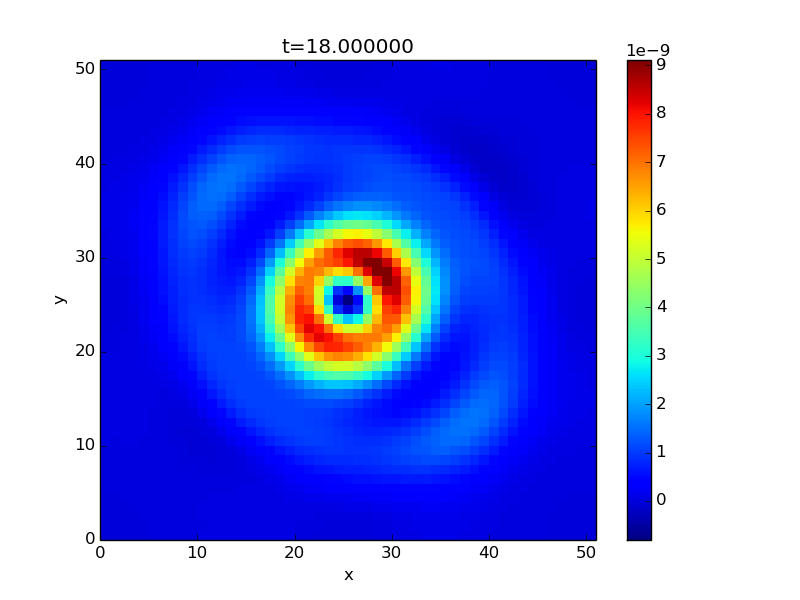
\includegraphics[width=4in]{shockwave}
		\caption{Energy distribution for a Gaussian source appearing with no dampening. The light blue ring is a wave of radiation generated by the sudden appearance of charge.}
		\label{fig:shockwave}
	\end{figure} 
	
	\begin{figure}
		\centering
		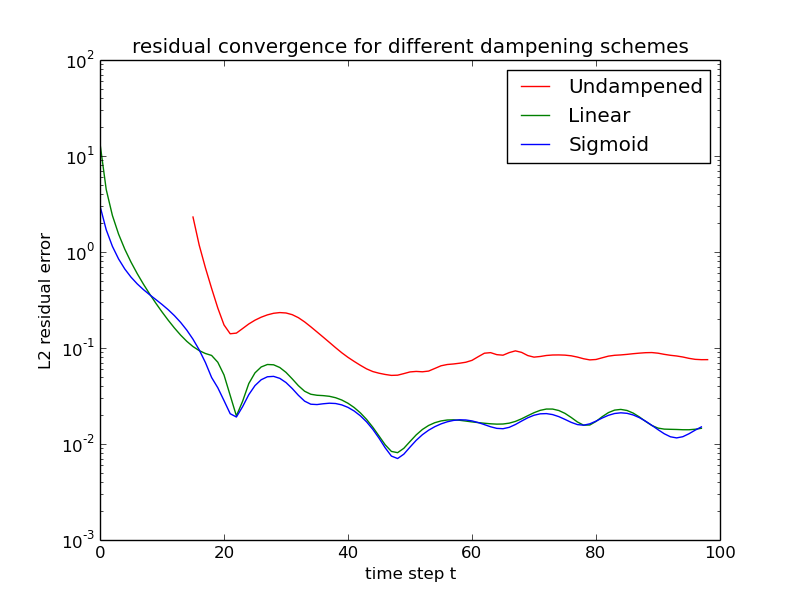
\includegraphics[width=4in]{conv_plot_100}
		\caption{L2 residual for different dampening schemes. Both the linear and the Sigmoid schemes start with no source at $t=0$ and ramp up to full strength at $t=20$. The undampened case is shifted to the right for comparison with the other schemes.}
		\label{fig:residual}
	\end{figure} 
	
	Even with the dampening, we still encountered some instability in our simulation. Since our source is radially symmetric, we would expect to see the same symmetry in our solution. However, there is some asymmetry, especially in $E_z$. This can be seen in Figure \ref{fig:asymmetry}. We are not exactly sure where this asymmetry comes from. Possibly our source is not perfectly centered when in position space. It also could be an error caused by the FFT.
	\begin{figure}
		\centering
		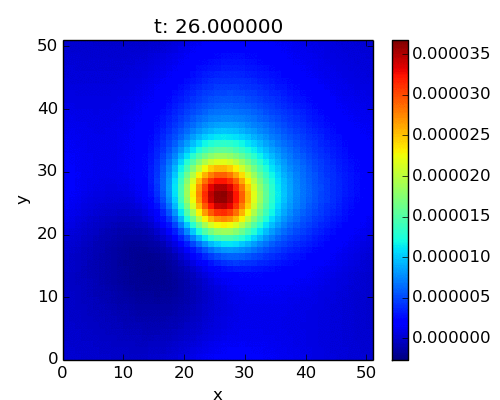
\includegraphics[width=4in]{asymmetry}
		\caption{Asymmetry in $E_z$ for a Gaussian with Sigmoid dampening. The electric field is noticeably greater in the top right quadrant compared to the other quadrants.}
		\label{fig:asymmetry}
	\end{figure} 

	
	Convergence: no analytic problem to compare to for the stable forms, so qualitatively compare the ``tail'' of the energy or electric field.
	
	\section{Simulations}
	
	mass dependence
	
	interesting charge sources
	
	interesting current sources
	
	\section{Conclusion}
	Summary of successes in relation to original goal
	
	Improvements
	
	What we would like to also implement
	
\end{document}